\item Reliability and availability:

\begin{itemize}
	\item textbf{Availability: }
	The Buzz system can be accessed at the following URL (http://buzz-codechat.rhcloud.com/) at any time of day on any of the widely used 	web browsers (Google Chrome, Mozilla Firefox, Microsoft Internet Explorer, Safari and Opera). The Buzz system even functions and displays 	correctly on the web browsers of mobile devices to ensure maximum availability.
	\item textbf{Reliability: }
	The system performs various error checks to ensure that no user action could cause the Buzz system to fail/crash (e.g. returning error messages if the user tries to log on with incorrect information , Figure 3). Even in cases were the system’s functionaity was not fully implemented procedures are in place to rather warn the user of incomplete operations instead of blindly carrying out a harmful request (e.g. an error message is diplayed when a user tries to upload a new profile picture, Figure4). The reason why the Buzz system can still function (to an extent) even though much of its functional procedures are incomplete/missing is due to the modular fashion in which the system was created. Even if one module of the system fails it is appropriatley seperated from the other modules to prevent a complete system failure.

\begin{figure}[h!]
  \centering
    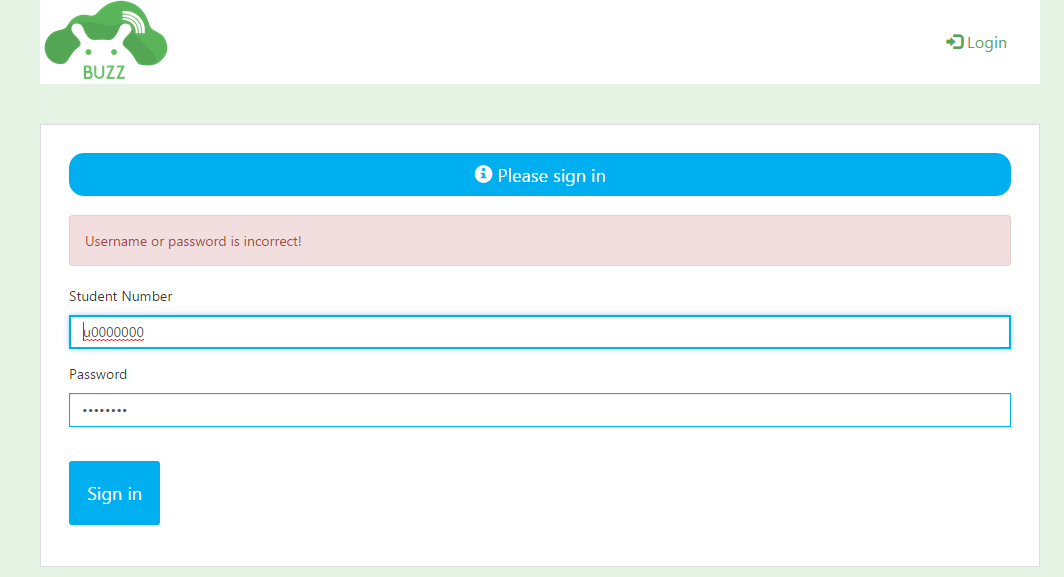
\includegraphics[width=0.85\textwidth]{ReliabilityB1}
    \caption{Login error}

\begin{figure}[h!]
  \centering
    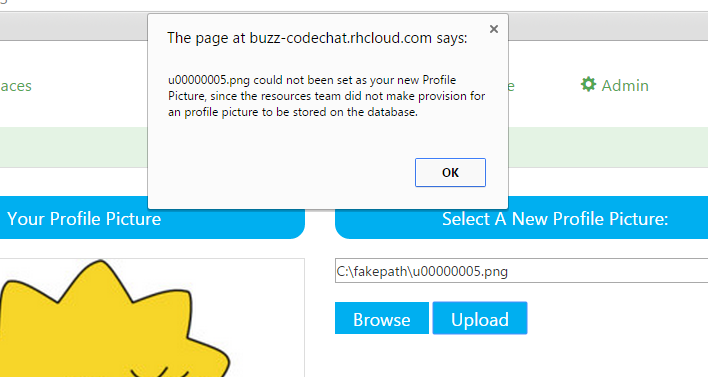
\includegraphics[width=0.85\textwidth]{ReliabilityB2}
    \caption{Error when uploading new profile picture}
\end{itemize}
	
